%%%%%%%%%%%%%%%%%%%%%%% preamble %%%%%%%%%%%%%%%%%%%%%%%%%%%
\documentclass[10pt,letterpaper]{article}
\usepackage{opex3}
%\usepackage{graphicx}
\usepackage{hyperref}
\usepackage{amssymb}
\hypersetup{colorlinks=true,
		      urlcolor=blue}
\usepackage{amsmath}      
\usepackage{bm}
\newcommand{\myeqno}[1]{Eq.~\eqref{#1}}
\DeclareMathOperator*{\argmin}{arg\,min}
%%%%%%%%%%%%%%%%%%%%%%% begin %%%%%%%%%%%%%%%%%%%%%%%%%%%%%%
%\linespread{1.25}
\begin{document}
\title{\Large{Assignment 3: Unsupervised learning}}
\author{\href{mailto:rohan.kekatpure@gmail.com}{Rohan D. Kekatpure}}
\address{}
\email{}

\begin{thebibliography}{9}
\bibitem{mnist} 
MNIST handwritten digit database.\\
\href{\tt http://yann.lecun.com/exdb/mnist/}{http://yann.lecun.com/exdb/mnist/}

\bibitem{ionosphere}
Ionosphere data at UCI.\\
\href{\tt https://archive.ics.uci.edu/ml/machine-learning-databases/ionosphere/ionosphere.names}{https://archive.ics.uci.edu/ml/machine-learning-databases/ionosphere/ionosphere.names}
\end{thebibliography}

\section{Description of the datasets}
This assignment asks us to apply five supervised learning algorithms on two datasets. The main goal of this exercise to understand the trade-offs in using these algorithms for real-world data mining and predictive modeling tasks. To accomplish this, one needs to identify non-trivial datasets rich in features and size to allow such comparative study. I have chosen the \href{http://yann.lecun.com/exdb/mnist/}{MNIST} \cite{mnist} and the \href{Its a binary classification problem allowing an easier comparative analysis of various learning algorithms.}{Ionosphere observations} \cite{ionosphere} datasets for my study. 

\subsection{What makes these datasets interesting?} 
The MNIST is a classic image recognition benchmark dataset consisting of 60000 labeled images of handwritten digits in the training set and 10000 in the testing set. Ionosphere observation dataset is 350 observations of 34 attributes with an objective to classify them into `good' `bad' observations --- classic binary classification problem. I believe the following factors qualify these datasets as `interesting':
%%
\subsubsection*{MNIST}
\begin{enumerate}
	\item It has been used to benchmark a number of learning algorithms in image recognition, allowing comparisions to published studies.
	\item Each training example is a $28\times28$ pixels image giving a dimensionality of 784. At this scale, dimensionality is expected to affect model performance making this dataset especially relevant for Assignment 3. 
	\item By using this dataset I'm taking the risk of not being able to perform training on the full dataset. Using dimensionality reduction helps us train on the full dataset, albeit with a reduced feature set. This once again highlights the utility of and need for dimensionality reduction.
\end{enumerate}
%%
\subsubsection*{Ionosphere}
For our studies, we include 150 observations in our training set and use the remaining 201 observations for testing. We don't know the train/test split use by the published studies, which might affect how closely we're able to reproduce these results.
\begin{enumerate}
	\item Ionosphere is a binary classification problem with 34 attributes. Its binary nature allows an easier comparative analysis of various binary classification algorithms.  
	\item A feature-set of size 34 should highlight some interesting aspects of dimensionality reduction. It is not as large as MNIST but not trivially small either. 
\end{enumerate}
%%
\section{Kmeans on MNIST dataset}
Using the {\tt stats} package in R, we performed K-means clustering on the MNIST dataset with $k=10$ and $k=20$. In a sense, the number of classes here is pre-decided by our domain knowledge. That is, we already know that we're classifying 10 handwritten digits. The question is how closely the cluster centers line up with identifiable digits. However, if our metric is training or test error, then we need to relax the $k=10$ constraint and study the error evolution as a function of $k$. Instead of the full evolution, here we perform clustering for only two values of $k$. 

For $k=10$ and $k=20$, the image representation of cluster centers is shown in Figure~\ref{kmeansfull}. For $k=10$, as shown in Fig~\ref{kmeansfull}(a), the centers largely seem to align with identifiable digits. However, because of the fixed number of classes, some digits seem to have merged (such as `4', `7' and `9'). Increasing $k$ to 20 seems to separate out the digits as shown in Fig~\ref{kmeansfull}(c). 
%%
\begin{figure}[tbp]
\begin{center}
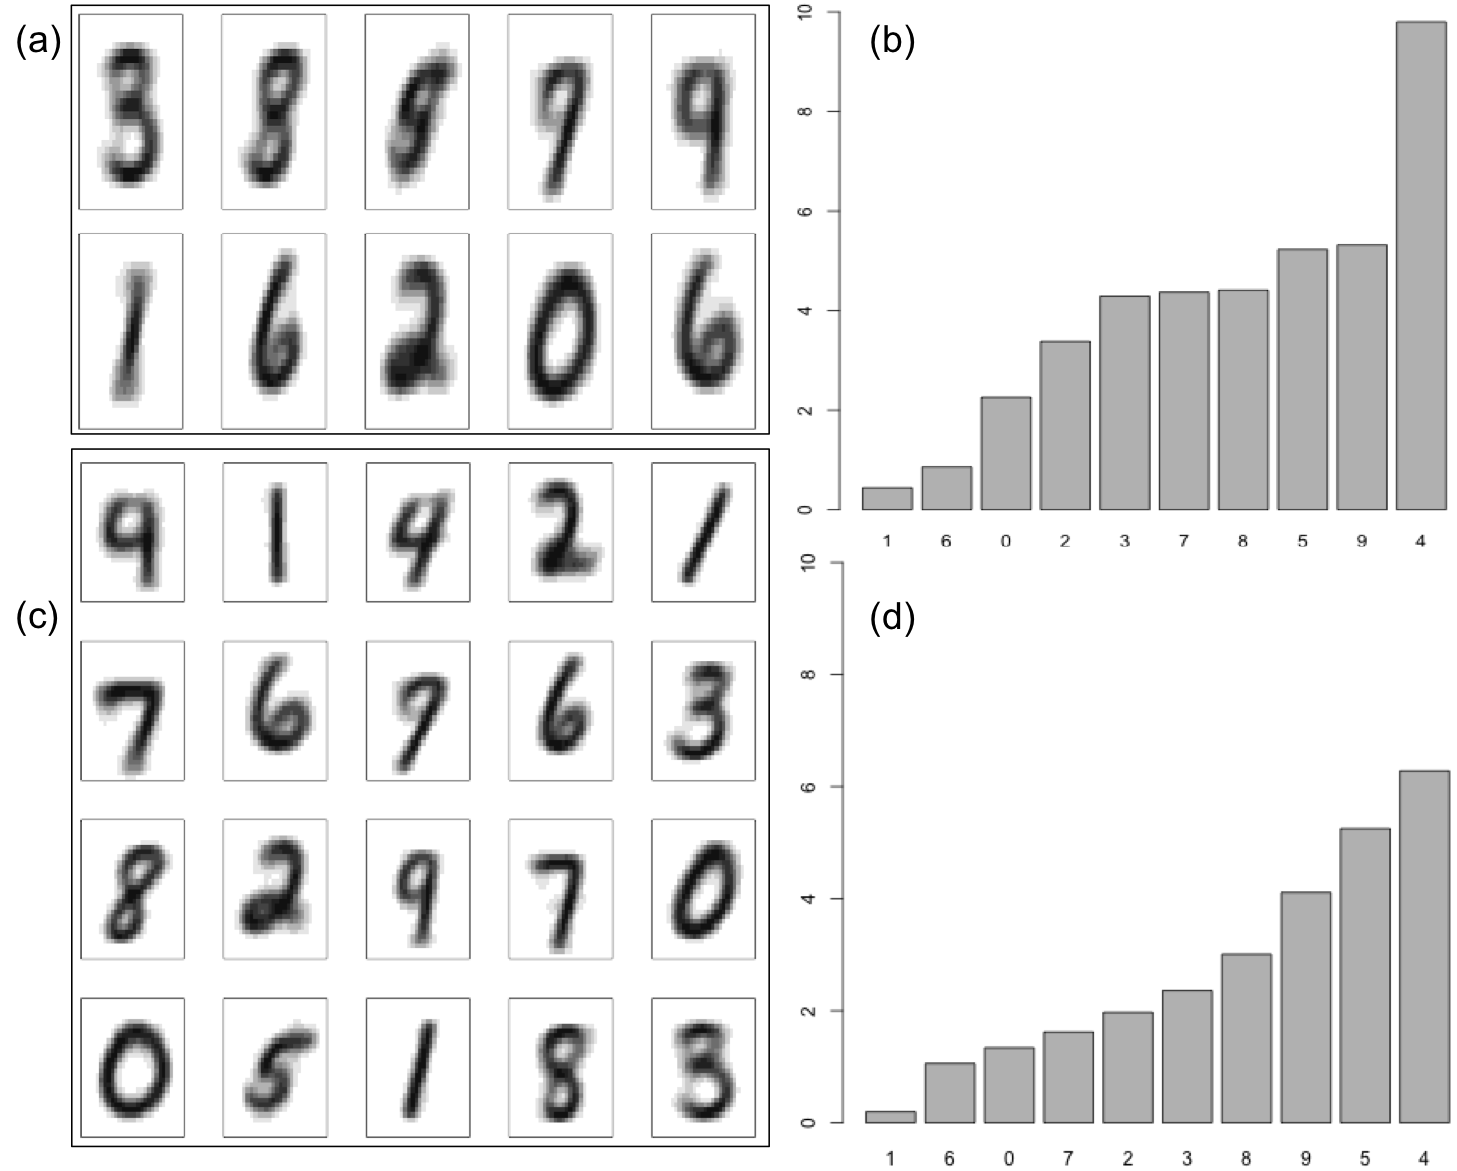
\includegraphics[width=4in]{../plots/kmeans.png}
\caption{Cluster centers and per-digit training error for MNIST data clustered using Kmeans clustering with $k=10$ (a, c) and $k=20$ (b, d)\label{kmeansfull}}
\end{center}
\end{figure}
%%
\subsection{How effective is Kmeans for classification}
This is fundamentally an image classification problem. So we also know the labels already. To study to effectiveness of Kmeans for classification task (a {\em supervised} learning problem) we computed training error by hand-assigning the classes to the returned clusters ({\tt c = [3,8,5,7,9,1,6,2,0,6]} for $k=10$ and {\tt c = [9,1,4,2,1,7,6,7,6,3,8,2,9,7,0,0,5,1,8,3]} for $k=20$). Notice the inherent subjectivity in the label assignment. The error are computed per digit for both $k = 10, 20$. The results are shown in Fig~\ref{kmeansfull}(b) and (d). For $k=10$, the maximum error is in identification of the digit `4' since there is no identifiable cluster corresponding to it. For $k=20$ the maximum error is for `8' and `3' since their corresponding clusters are intermixed. 
\begin{table}[tbp]
    \begin{center}
        \begin{tabular}{c|c|c}
            \hline
            {\bf Training set size}&{\bf \# of clusters}&{\bf Avg classification error} \\ \hline
            10000&10&40.36\% \\
            10000&20&27.20\% \\ \hline
            \end{tabular}
            \caption{Average training error in detection of digits in the MNIST database using KMeans algorithm. \label{tab1} }
        \end{center}
\end{table}
Overall, Kmeans is an effective technique to visualize the clusters in the MNIST dataset, but is not sufficient by itself for the classification task.
\section{Expectation maximization on MNIST}
We repeated the same experiment as above, but with Expectation Maximization (EM) as our clustering algorithm. The results are shown in Fig~\ref{emfull}. The general observations for EM algorithm as well as its treatment for classification are similar to Kmeans. One difference is that EM algorithms requires more training time due to more involved Bayesian inversion as opposed to simply calculating means in Kmeans. As a result, the EM algorithm was run on a sample size that was 1/10th the size for KMeans. Table 
%%
\begin{figure}[tbp]
\begin{center}
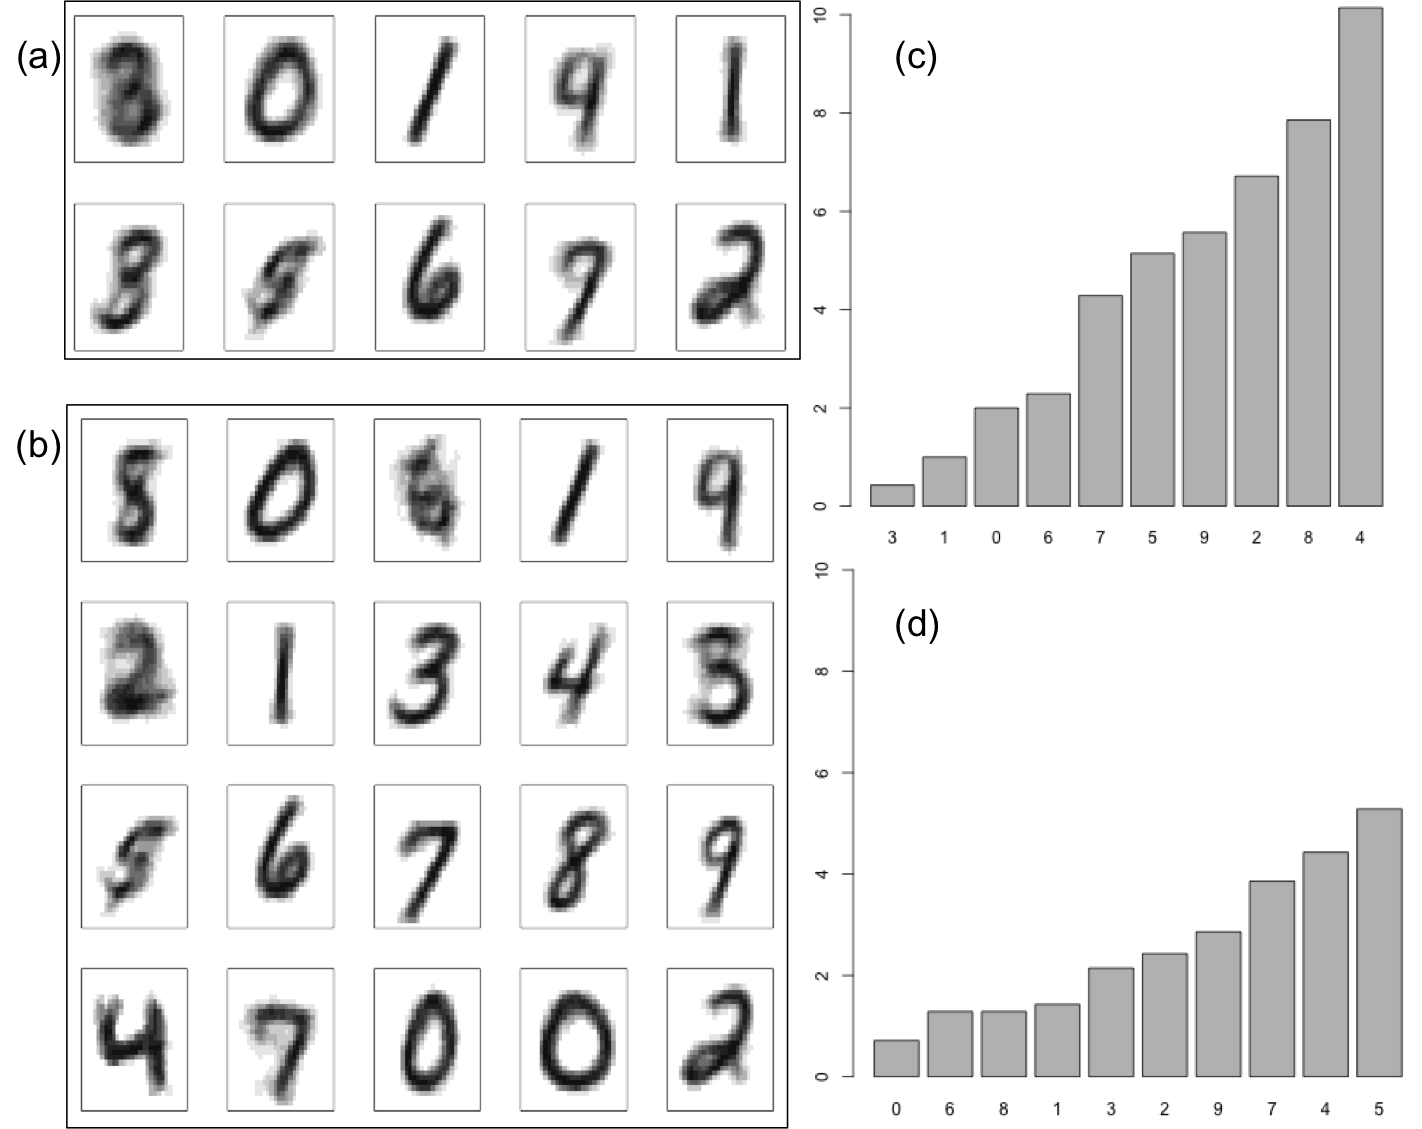
\includegraphics[width=4in]{../plots/exmax.png}
\caption{Cluster centers and per-digit training error for MNIST data clustered using EM clustering with $k=10$ (a, c) and $k=20$ (b, d)\label{emfull}}
\end{center}
\end{figure}
%%
\begin{table}[tbp]
    \begin{center}
        \begin{tabular}{c|c|c}
            \hline
            {\bf Training set size}&{\bf \# of clusters}&{\bf Avg classification error} \\ \hline
            1000&10&41.29\% \\
            1000&20&29.12\% \\ \hline
            \end{tabular}
            \caption{Average training error in detection of digits in the MNIST database using the EM algorithm. \label{tab2} }
        \end{center}
\end{table}
%%
%%
\section{PCA on MNIST}
Next we applied Principal Components Analysis (PCA) on the MNIST training set. The dimension of the original feature space for the MNIST dataset is 784. PCA essentially rotates this input space and ranks the new co-ordinate directions by the amount of variance present along each. We can then choose to retain the number of principal components required to achieve a certain test error.

We ran the PCA on 10000 rows of the MNIST training set. Figure~\ref{pcacoverage} plots the cumulative variance captured by addition of each individual principal component. As shown by the red line, 150 components are required to cover 95\% variance. The number 95\% is arbitrary and a rough guideline only; it does not mandate that our new training set must contain 150 components. The ultimate test is the training and the test error we get by applying a learning algorithm on the reduced dimensionality set. 
%
\begin{figure}[tbp]
\begin{center}
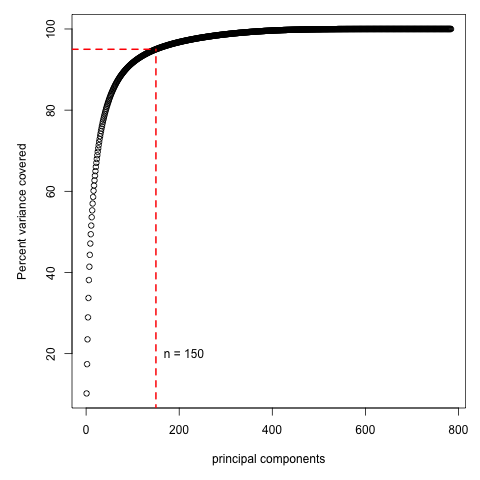
\includegraphics[width=2.5in]{../plots/pcacoverage.png}
\caption{Cumulative variance covered by the successive PCA components for the MNIST dataset. \label{pcacoverage}}
\end{center}
\end{figure}
%
%
%
\begin{figure}[tbp]
    \begin{center}
    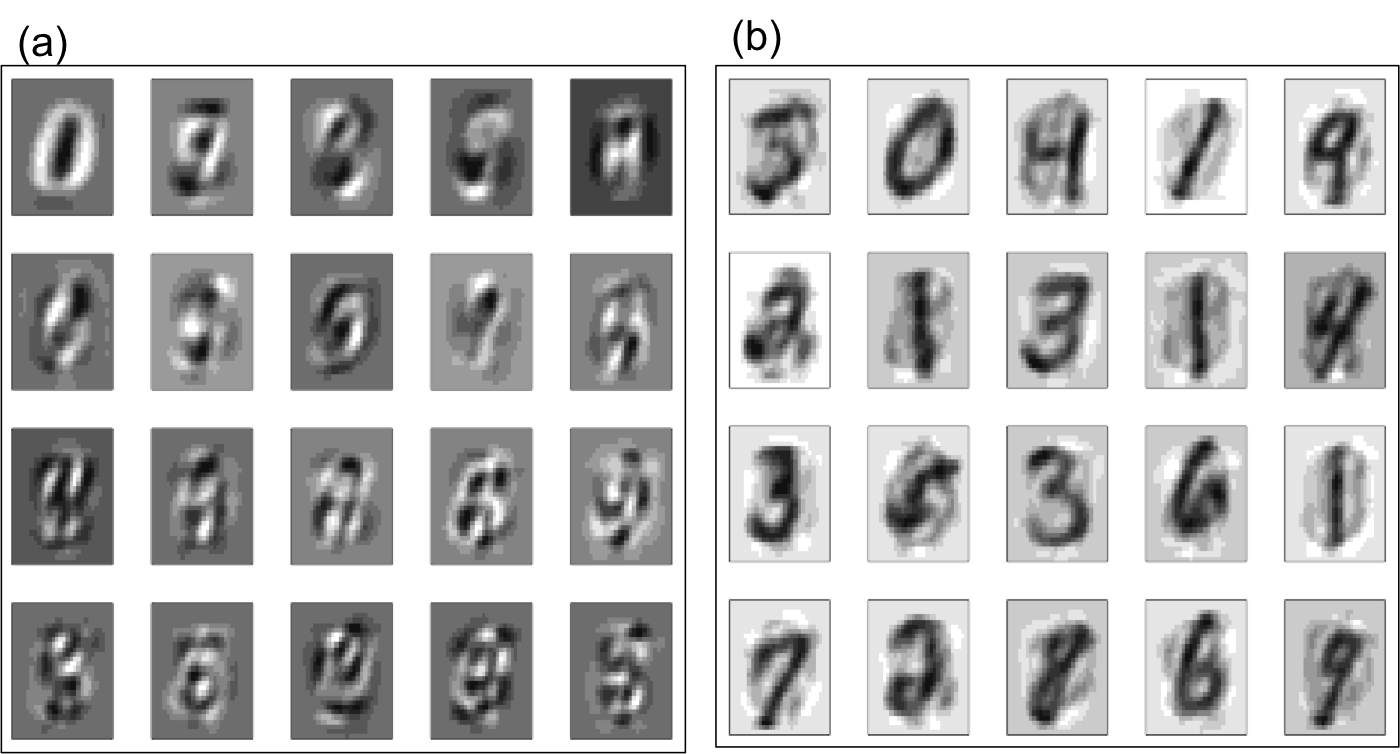
\includegraphics[width=4in]{../plots/pca.png}
    \caption{(a) Selected singular vectors of the MNIST database. Reading from left to right the plotted principal components are 1--15, 20, 30, 40, 50 and 100. (b) Reconstruction of the original data using the first 25 principal components. \label{pcainsight}}
    \end{center}
\end{figure}
%
For a further insight into PCA, we plotted 20 Singluar vectors (1--15, 20, 30, 40, 50 and 100) of the MNIST database in Fig~\ref{pcainsight}(a) and a reconstruction of the original data using the first 25 principal components in Fig~\ref{pcainsight}{b}. As expected from the PCA theory the successive principal components become more pixelated, signifying more positive-to-negative crossings and thereby more variance. For sufficiently high orders, the principals components are hard to distinguish from noise and justifying their exclusion from analysis. 

Fig~\ref{pcainsight}(b) shows that as few as 25 components are sufficient for reconstructing identifiable digits. Later we'll be presenting neural network test error as a function of number of Principal components.
\section{ICA on MNIST}
We ran ICA on the MNIST dataset using the {\tt ICA} package in R. The total kurtosis for the first 100 components is plotted in Fig~\ref{icadist}. As expected the algorithm has found highly kurtotic components under the assumption of independence. 
%
\begin{figure}[bp]
    \begin{center}
    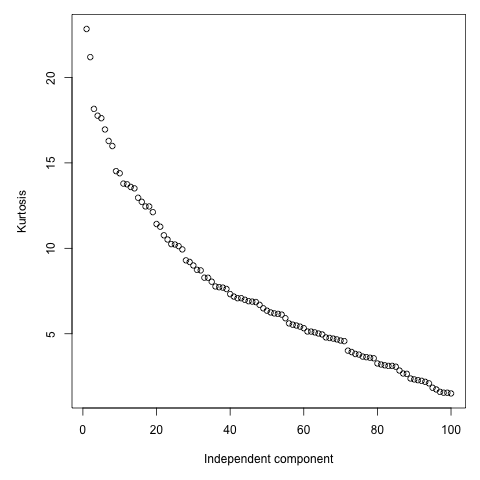
\includegraphics[width=2.5in]{../plots/icadist.png}
    \caption{Kurtosis of the first 100 ICA components for the MNIST dataset \label{icadist}}
    \end{center}
\end{figure}
%
\section{PCA + KMeans}
We ran KMeans clustering on the data after retaining the first 10 PCA components. Since the clusters cant be visualized as digits after dimensionality reduction, the question of how similar the clusters are before and after dimensionality reduction needs to be considered carefully. To measure similarity, we use the Jaccard index. That is, we ask, "how many observations have remained in the same cluster even after dimensionality reduction?" We compute this per digit. Our results are summarized in the table below. 
\begin{table}[tbp]
\begin{center}
\begin{tabular}{c|c|c }
\hline
{\bf cluster before DR}&{\bf cluster after DR}&{\bf similarity} \\ \hline
1 &3&99.28 \\
2 & 7& 98.43\\
3 &6&81.29 \\
4&2&86.21\\
5&10&98.05\\
6&4&92.19\\
7&9&89.06\\
8&1&98.77\\
9&8&87.97\\
10&5&82.06\\ \hline
\end{tabular}
\end{center}
\caption{Cluster similarity with PCA + KMeans with 10 PCA components. \label{kmpca}}
\end{table}
Most training examples stayed with their original clusters after dimensionality reduction. Some examples (for example original cluster \# 3) shifted more. If we look at the original cluster \# 3 in Fig~\ref{kmeansfull}, the membership of that cluster is hard to ascertain.
%%
\section{PCA + Expectation maximization}
\begin{table}[tbp]
\begin{center}
\begin{tabular}{c|c|c }
\hline
{\bf cluster before DR}&{\bf cluster after DR}&{\bf similarity} \\ \hline
 1 & 6 & 92.10\\ 
 2 & 2 & 100.00\\ 
 3 & 3 & 100.00\\ 
 4 & 9 & 100.00\\ 
 5 & 5 & 97.32\\ 
 6 & 8 & 95.00\\ 
 7 & 7 & 100.00\\ 
 8 & 1 & 100.00\\ 
 9 & 4 &92.29\\ 
 10 & 10 & 100.00 \\ \hline 
\end{tabular}
\end{center}
\caption{Cluster similarity with PCA + EM with 10 PCA components. \label{empca}}
\end{table}
%%
Dimensionality reduction does not appear to affect cluster membership calculated by the EM algorithm as much as it does KMeans. The maximum-likelihood-based approach potentially makes the algorithm more robust compared to KMeans (this is just an hypothesis that'll need to be more carefully investigated with more experiments).
%%
\section{ICA + KMeans}
Repeating the same experiment, and the same similarity definition as before for ICA + KMeans we obtain the following table of before/after cluster memberships.
%%
\begin{table}[tbp]
\begin{center}
\begin{tabular}{c|c|c }
\hline
{\bf cluster before DR}&{\bf cluster after DR}&{\bf similarity} \\ \hline
1 & 6 & 85.238095\\
2 & 8 & 93.457944\\
3 & 4 & 97.826087\\
4 & 3 & 87.500000\\
5 & 9 & 96.491228\\
6 & 5 & 97.979798\\
7 & 6 & 91.794872\\
8 & 3 & 93.085106\\
9 & 5 & 82.905983\\
10 & 2 & 98.924731 \\ \hline
\end{tabular}
\end{center}
\caption{Cluster similarity with ICA + KMeans with 10 ICA components. \label{kmica}}
\end{table}
Note that original clusters 1 and 7 in this case are mapped to cluster 6 in the post DR set. But the overall cluster membership has been retained at a fairly high percentage.
%%
\section{ICA + EM}
\begin{table}[tbp]
\begin{center}
    \begin{tabular}{c|c|c }
    \hline
    {\bf cluster before DR}&{\bf cluster after DR}&{\bf similarity} \\ \hline
        1 & 9 & 79.234973\\ 
        2 & 2 & 99.047619\\ 
        3 & 4 & 97.727273\\ 
        4 & 5 & 96.000000\\ 
        5 & 7 & 100.000000\\ 
        6 & 9 & 70.454545\\ 
        7 & 10 & 76.923077\\ 
        8 & 8 & 93.333333\\ 
        9 & 9 & 97.222222\\ 
        10 & 6 & 98.437500 \\ \hline
    \end{tabular}
\end{center}
\caption{Cluster similarity with ICA + EM with 10 ICA components. \label{kmica}}
\end{table}
EM with ICA does not display the same robustness in before/after cluster membership as it did with PCA. One possible cause of this may be that the reduced dimensionality representation of the MNIST dataset using PCA is more accurate than ICA. 
\section{PCA + Neuralnet}
We ran the NN from assignment 1 (1 hidden layer, 50 hidden units) by feeding, respectively, 95, 43, 19, and 9 principal components. Also, for this and all the following neural network experiments, the training set size was 500 and the test set size was 10000 samples. 

For the PCA + neural net, the variation of the training time, training error and the test error is shown in Table~\ref{pcann}
\begin{table}[tbp]
\begin{center}
    \begin{tabular}{c|c|c |c}
    \hline
    {\bf \# Components}&{\bf training error \%}&{\bf test error\%} & {\bf run time (sec)} \\ \hline
	95 & 0.0 & 11.34 & 100 \\
	43 & 0.0 & 10.53 & 22 \\
	19 & 0.0 & 11.88 & 8 \\
	9 & 0.0 & 15.18 & 3 \\ \hline
    \end{tabular}
\end{center}
\caption{Performance of neural net + PCA \label{pcann}}
\end{table}
%
The data in Table~\ref{pcann} suggest that running a model with only 20 components gives the same performance on the test set in a substantially lesser time. Moreover, pre-smoothening the dataset with PCA also reduces overfitting. 

\section{ICA + Neuralnet}
As with PCA, we looped through the number of independent components for ICA and computed the training and the test set error of the neural network. Our results are reported in Table~\ref{icann}.
\begin{table}[tbp]
\begin{center}
    \begin{tabular}{c|c|c |c}
    \hline
    {\bf \# Components}&{\bf training error \%}&{\bf test error\%} & {\bf run time (sec)} \\ \hline
 10  & 0.200000  & 33.390000  & 2.772000\\ 
 20  & 0.000000  & 23.740000  & 6.389000\\ 
 30  & 0.000000  & 24.400000  & 11.262000\\ 
 40  & 0.000000  & 20.180000  & 17.538000\\ 
 50  & 0.000000  & 23.790000  & 25.594000\\ 
 60  & 0.000000  & 25.310000  & 34.456000\\ 
 70  & 0.000000  & 22.510000  & 47.097000\\ 
 80  & 0.000000  & 22.170000  & 61.531000 \\ \hline
    \end{tabular}
\end{center}
\caption{Performance of neural net + ICA \label{icann}}
\end{table}

The performance of Neural net with ICA is considerably worse compared to PCA (10\% vs 20\% test error). ICA's central assumption is that the total signal is a linear sum of statistically independent sources. However, for MNIST data, the statistical independence of consecutive (or even far removed) pixels can be questioned. It can be argued that in text images, there are likely to be continuous streaks of similarly valued pixels. 

Overall, the worse performance of Neuralnet + ICA may be stemming from ICA not being the right dimensionality reduction technique for digitized handwritten text data. 


\section{KMeans + Neuralnet}
After obtaining the clusters using KMeans, one needs to define a way to extract the reduced feature set from the clusters. There are multiple options. We can calculate distance to the cluster centers, or the dot product with the unit vectors in the directions of the clusters. However, ignoring the magnitude of the sample and depending only on the direction seems less optimal. So we calculate our reduced feature set from KMeans using `distance to cluster centers' method. We varied the number of clusters and computed the training and the test set error. The results are reported in Table~\ref{kmnn}
\begin{table}[bp]
\begin{center}
    \begin{tabular}{c|c|c |c}
    \hline
    {\bf \# Clusters}&{\bf training error \%}&{\bf test error\%} & {\bf run time (sec)} \\ \hline
  10  &  1.400000  &   25.140000  &   3.103000\\ 
  30  &  0.000000  &   18.140000  &   12.000000\\ 
  50  &  0.000000  &   15.940000  &   26.353000\\ 
  70  &  0.000000  &   16.370000  &   47.841000\\ 
  90  &  0.000000  &   15.470000  &   79.926000 \\ \hline
\end{tabular}
\end{center}
\caption{Performance of neural net + KMeans \label{kmnn}}
\end{table}
The results are reasonable considering the simplicity and computational cost of the KMeans relative to PCA. However, there seems to be no straightforward way to improve the performance of KMeans as a dimensionality reduction technique. It is preferable to have a trade-off between computational cost (run time) and accuracy and KMeans does not seem to offer that. 

\end{document}













